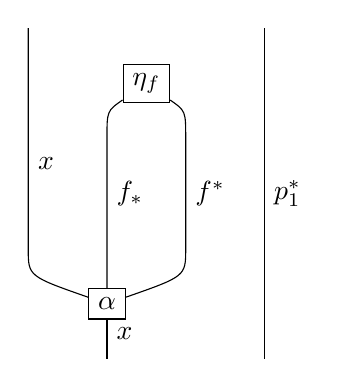
\begin{tikzpicture}[baseline=(current bounding box.center),y=0.7cm]
\path coordinate[] (tikzsd_internal_pos_0_0) at (0.0,0.0);
\path coordinate[] (tikzsd_internal_pos_0_1) at (3.0,0.0);
\path coordinate[] (tikzsd_internal_pos_1_0) at (0.0,-2.0);
\path coordinate[] (tikzsd_internal_pos_1_1) at (1.0,-2.0);
\path coordinate[] (tikzsd_internal_pos_1_2) at (2.0,-2.0);
\path coordinate[] (tikzsd_internal_pos_1_3) at (3.0,-2.0);
\path coordinate[] (tikzsd_internal_pos_2_0) at (0.0,-4.0);
\path coordinate[] (tikzsd_internal_pos_2_1) at (1.0,-4.0);
\path coordinate[] (tikzsd_internal_pos_2_2) at (2.0,-4.0);
\path coordinate[] (tikzsd_internal_pos_2_3) at (3.0,-4.0);
\path coordinate[] (tikzsd_internal_pos_3_0) at (1.0,-6.0);
\path coordinate[] (tikzsd_internal_pos_3_1) at (3.0,-6.0);

\path node[,draw,] (tikzsd_internal_nt_node_0_0) at (1.5,-1.0) {$\eta_f$};
\path node[,draw,] (tikzsd_internal_nt_node_2_0) at (1.0,-5.0) {$\alpha$};

\path [draw] (tikzsd_internal_pos_0_0) ..controls(0.0,-0.5)and(0.0,-1.5)..(tikzsd_internal_pos_1_0) ..controls(0.0,-2.5)and(0.0,-3.5)..(tikzsd_internal_pos_2_0) node[pos=0.25,auto,] {$x$} ..controls(0.0,-4.5)..(tikzsd_internal_nt_node_2_0);
\path [draw] (tikzsd_internal_nt_node_0_0) ..controls(1.0,-1.5)..(tikzsd_internal_pos_1_1) ..controls(1.0,-2.5)and(1.0,-3.5)..(tikzsd_internal_pos_2_1) node[pos=0.5,auto,] {$f_\ast$} ..controls(1.0,-4.5)..(tikzsd_internal_nt_node_2_0);
\path [draw] (tikzsd_internal_nt_node_0_0) ..controls(2.0,-1.5)..(tikzsd_internal_pos_1_2) ..controls(2.0,-2.5)and(2.0,-3.5)..(tikzsd_internal_pos_2_2) node[pos=0.5,auto,] {$f^\ast$} ..controls(2.0,-4.5)..(tikzsd_internal_nt_node_2_0);
\path [draw] (tikzsd_internal_nt_node_2_0) ..controls(1.0,-5.5)..(tikzsd_internal_pos_3_0) node[pos=0.5,auto,] {$x$};
\path [draw] (tikzsd_internal_pos_0_1) ..controls(3.0,-0.5)and(3.0,-1.5)..(tikzsd_internal_pos_1_3) ..controls(3.0,-2.5)and(3.0,-3.5)..(tikzsd_internal_pos_2_3) node[pos=0.5,auto,] {$p_1^\ast$} ..controls(3.0,-4.5)and(3.0,-5.5)..(tikzsd_internal_pos_3_1);
\end{tikzpicture}